\newcommand{\figureShiftRegisterSIPO}[1]{
  \def\lang{\detokenize{#1}}
  \def\langRu{\detokenize{ru}}
  \def\langEn{\detokenize{en}}
  \def\figureCaption{XXX: No translation.}
  \ifx \lang\langRu
  \def\figureCaption{
    Распиновка последовательно-параллельного сдвигового регистра 74HC595.
  }
  \fi
  \ifx \lang\langEn
  \def\figureCaption{
    Pinout of serial-in/parallel-out shift register 74HC595.
  }
  \fi
  \begin{figure}[ht]
    \centering
    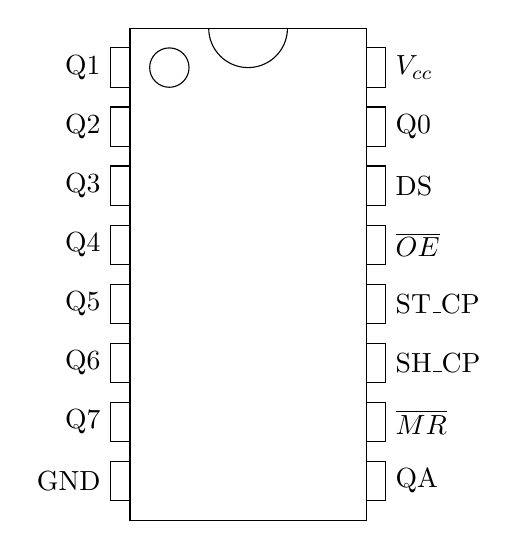
\begin{tikzpicture}
      %%%% Rectangles.
      \draw (0, 1.75) rectangle (3, 8);
      \foreach \ys/\ye in {
        7.75/7.25,              % Q1
        7.00/6.50,              % Q2
        6.25/5.75,              % Q3
        5.50/5.00,              % Q4
        4.75/4.25,              % Q5
        4.00/3.50,              % Q6
        3.25/2.75,              % Q7
        2.50/2.00               % GND
      } {
        \draw (-0.25, \ys) rectangle (0, \ye);
        \draw (3.00, \ys) rectangle (3.25, \ye);
      }
      %%%% Keys
      \draw (1.0, 8.0) arc [start angle=180, end angle=360, radius=0.5cm];
      \draw (0.75, 7.50) arc [start angle=0, end angle=360, radius=0.25cm];
      %%%% Text.
      %% Left side:
      \node[anchor=east] at (-0.25, 7.50) {Q1};
      \node[anchor=east] at (-0.25, 6.75) {Q2};
      \node[anchor=east] at (-0.25, 6.00) {Q3};
      \node[anchor=east] at (-0.25, 5.25) {Q4};
      \node[anchor=east] at (-0.25, 4.50) {Q5};
      \node[anchor=east] at (-0.25, 3.75) {Q6};
      \node[anchor=east] at (-0.25, 3.00) {Q7};
      \node[anchor=east] at (-0.25, 2.25) {GND};
      %% Right side:
      \node[anchor=west] at (3.25, 7.50) {$V_{cc}$};
      \node[anchor=west] at (3.25, 6.75) {Q0};
      \node[anchor=west] at (3.25, 6.00) {DS};
      \node[anchor=west] at (3.25, 5.25) {$\overline{OE}$};
      \node[anchor=west] at (3.25, 4.50) {ST\_CP};
      \node[anchor=west] at (3.25, 3.75) {SH\_CP};
      \node[anchor=west] at (3.25, 3.00) {$\overline{MR}$};
      \node[anchor=west] at (3.25, 2.25) {QA};
    \end{tikzpicture}
    \caption{\figureCaption}
    \label{fig:shift-register-sipo}
  \end{figure}
}
